\chapter{Технологическая часть}

В данном разделе будет представлена реализация решения поставленной задачи в формате листинга кода. Также будут указаны требования к ПО и средства реализации, описан пользовательский интерфейс и
результаты проведенного тестирования программы.

\section{Требования к ПО}

Были учтены следующие требования к программе:
\begin{enumerate}[label=\arabic*)]
    \item Программа выводит сообщение об ошибке и генерирует ненулевой код
возврата в случае возникновения исключения в процессе выполнения.
    \item Программа выполняет построение изображения сцены из трехмерных
объектов.
    \item Программа выполняет обработку только многогранников, геометрия
которых описана с помощью $obj$ файла.
    \item Программа принимает на вход файлы, составленные по правилам, которые описаны ниже.
    \item Программа может сохранять полученное изображение в $png$ файл.
    \item Программа предоставляет возможность отрисовывать анимацию дождя.
    \item Программа предоставляет возможность отрисовывать анимацию молний.
    
\end{enumerate} 

\section{Требования к входным данным}
Требования к входному файлу:
\begin{enumerate}[label=\arabic*)]
\item На вход принимаются только $obj$ файлы.
\item Модели в файле должны быть триангулированы.
\item Описание каждой модели начинается с буквы $o$.
\end{enumerate} 

\section{Средства реализации}

В качестве языка программирования для разработки ПО был выбран
язык программирования $C++$\cite{cpp}. Данный выбор обусловлен наличием
необходимого функционала для работы с наборами объектов. Также был
выбран фреймворк $Qt$\cite{qt} в связи с наличием необходимых для работы с
компьютерной графикой библиотек и встроенных средств.

Для хранения информации о многогранниках, заданных при помощи полигональной сетки, были использованы $obj$ файлы. Данный выбор
обусловлен тем, что $obj$ является одним из самых популярных форматов
передачи трехмерной компьютерной геометрии\cite{obj}. Для хранения полученного изображения был выбран формат $png$, так как среднеквадратическая
ошибка — среднее различие в квадрате между идеальным и фактическим
пиксельными значениями — для, например, $jpeg$ файлов на больших изображениях гораздо больше, чем у $png$ файлов \cite{png}, и качество изображения
формата $png$ не меняется при любой степени сжатия.

\section{Реализация разработанного ПО}

В приведенных ниже листингах представлены следующие реализации:
\begin{enumerate}[label=\arabic*)]
    \item модифицированный алгоритм $Z$-буфера (листинг \ref{zb});
    \item алгоритм простой закраски (листинг \ref{simple});
    \item алгоритм генерации молнии (листинг \ref{lightning}).
\end{enumerate}
\clearpage
\begin{lstlisting}[firstnumber=1,caption={Реализация модифицированного алгоритма $Z$-буфера}, label=zb]
void ZBuffer::putPolygon(std::vector<QVector3D> &points,
                         std::vector<LightSource> &ls, QColor c,
                         std::vector<std::vector<std::vector<double>>> &shadows) {
  int ymax, ymin, xmax, xmin;
  ymax = ymin = points[0].y();
  xmax = xmin = points[0].x();
  for (size_t i = 1; i < points.size(); i++) {
    int x = points[i].x();
    int y = points[i].y();
    if (y > ymax)
      ymax = y;
    else if (y < ymin)
      ymin = y;
    if (x > xmax)
      xmax = x;
    else if (x < xmin)
      xmin = x;
  }
  ymin = (ymin < 0) ? 0 : ymin;
  ymax = (ymax < _sY) ? ymax : _sY - 1;
  xmin = (xmin < 0) ? 0 : xmin;
  xmax = (xmax < _sX) ? xmax : _sX - 1;
  std::tuple<int, int, int, int> coef = planeCoef(points);
  QVector3D N(std::get<0>(coef), std::get<1>(coef), std::get<2>(coef));
  N.normalize();
  if (QVector3D::dotProduct(N,QVector3D(0, 0, 5000)) < 0)
      N *= (-1);
  for (int i = xmin; i <= xmax; i++)
    for (int j = ymin; j <= ymax; j++) {
      if (isInside(i, j, points)) {
        double z = calculateZ(i, j, coef);
        if (z > _buf[i][j].z) {
          _buf[i][j].z = z;
          _buf[i][j].c = calculateColor(i,j,z, N, ls, c, shadows);
        }
      }
    }
}

\end{lstlisting}
\clearpage
\begin{lstlisting}[firstnumber=1,caption={Реализация алгоритма простой закраски}, label=simple]
QColor calculateColor(int x, int y, double z,
                      QVector3D N,
                      std::vector<LightSource> ls, QColor c,
                      std::vector<std::vector<std::vector<double>>> &shadows) {
    QVector3D point(x,y,z);
    double diffuse_light_intensity = 0;
      for (size_t i=0; i<ls.size(); i++) {
          QVector3D light_dir      = (ls[i].getPos() - point);
         if (light_dir.length() > shadows[i][x][y])
             continue;
          light_dir.normalize();
          diffuse_light_intensity  += ls[i].getIntensity() * std::max(0.f, QVector3D::dotProduct(light_dir,N));
      }
   QVector3D cv(c.red() / 255, c.green() / 255, c.blue() / 255);
   cv = cv * diffuse_light_intensity;
   QColor color = QColor(255 * std::max(0.f, std::min(1.f, cv.x())), 255 * std::max(0.f, std::min(1.f, cv.y())), 255 * std::max(0.f, std::min(1.f, cv.z())));

  return color;
}

\end{lstlisting}
\clearpage
\begin{lstlisting}[firstnumber=1,caption={Реализация алгоритма генерации молнии}, label=lightning]
void Lightning::generateLightning(QPoint &point1, QPoint &point2)
{
    _branches.clear();
    int mx_var = sqrt((point1.x() - point2.x()) * (point1.x() - point2.x()) + (point1.y() - point2.y()) * (point1.y() - point2.y())) / 2;
    if (mx_var < MIN_DIST) mx_var = 15;
    _branches.push_back(line_t{point1, point2});
    int k = 3 + rand() % 8;
    for(int i = 0; i < k && i < _branches.size(); i++){
        QVector2D p1 = QVector2D(_branches[i].p1.x(), _branches[i].p1.y());
        QVector2D p2 = QVector2D(_branches[i].p2.x(), _branches[i].p2.y());
        _branches.erase(_branches.begin() + i);
        QVector2D mid = (p1 + p2) / 2;
        if ((mid - p1).length() < MIN_DIST){
            _branches.push_back({QPoint(p1.x(), p1.y()), QPoint(p2.x(), p2.y())});
            break;
        }
        QVector2D N(p2.y() - p1.y(), -(p2.x() - p1.x()));
        N.normalize();
        bool flag = rand()%2;
        if (flag){
            mid += N * (7 + rand()%5);
            QVector2D newPoint(mid.x() + 2 + rand()%80, mid.y() + 2 + rand()%80);
            _branches.push_back({QPoint(newPoint.x(), newPoint.y()), QPoint(mid.x(), mid.y())});
        }
        else mid -= N * (7 + rand()%5);
        _branches.push_back({QPoint(p1.x(), p1.y()), QPoint(mid.x(), mid.y())});
        _branches.push_back({QPoint(mid.x(), mid.y()), QPoint(p2.x(), p2.y())});
        if ((mid - p1).length() < 3 * MIN_DIST) continue;
        i--;
    }
}
\end{lstlisting}

\section{Интерфейс программы}

Программа запускается с помощью среды разработки $QtCreator$ при
нажатии на кнопку сборки и запуска в левом нижнем углу.

На рисунке \ref{img:interface} представлен пользовательский интерфейс разработанной программы.

\begin{figure}[H]
	\centering
	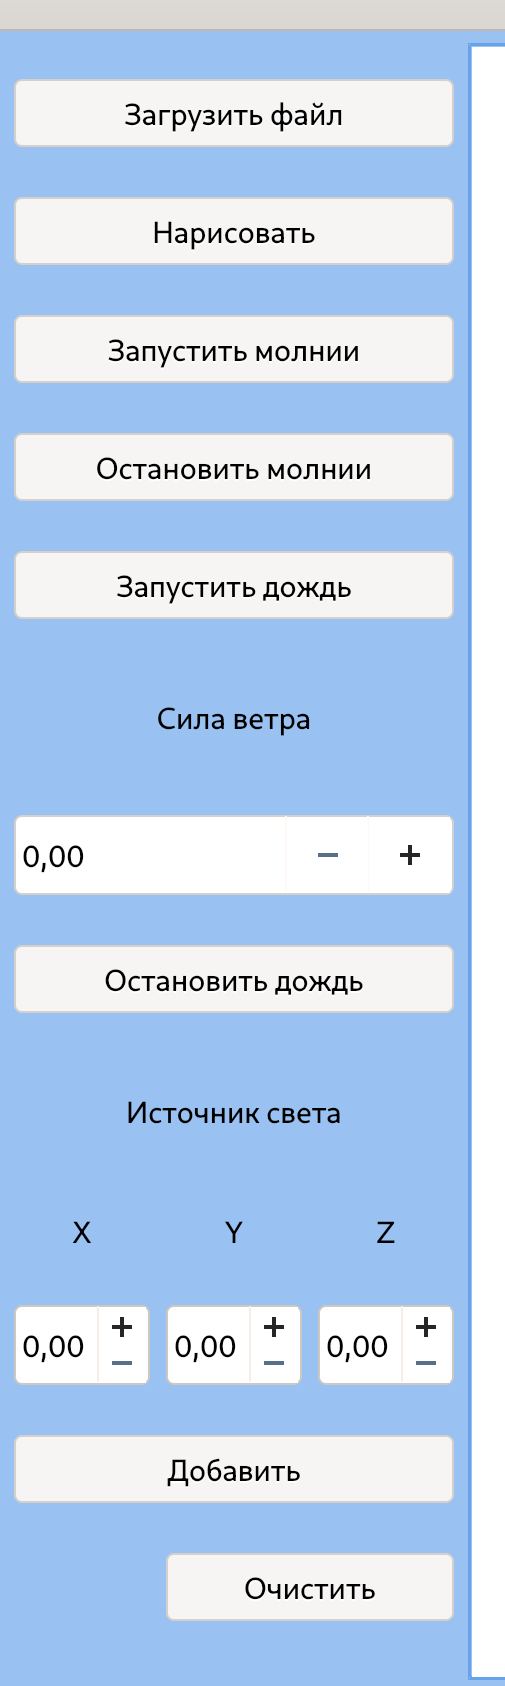
\includegraphics[scale=0.3]{include/inerface.png}
	\caption{Интерфейс программы}
	\label{img:interface}
\end{figure} 

\section{Примеры работы программы}

На рисунках \ref{img:1} — \ref{img:7} представлены примеры работы реализованной
программы.

\begin{figure}[H]
	\centering
	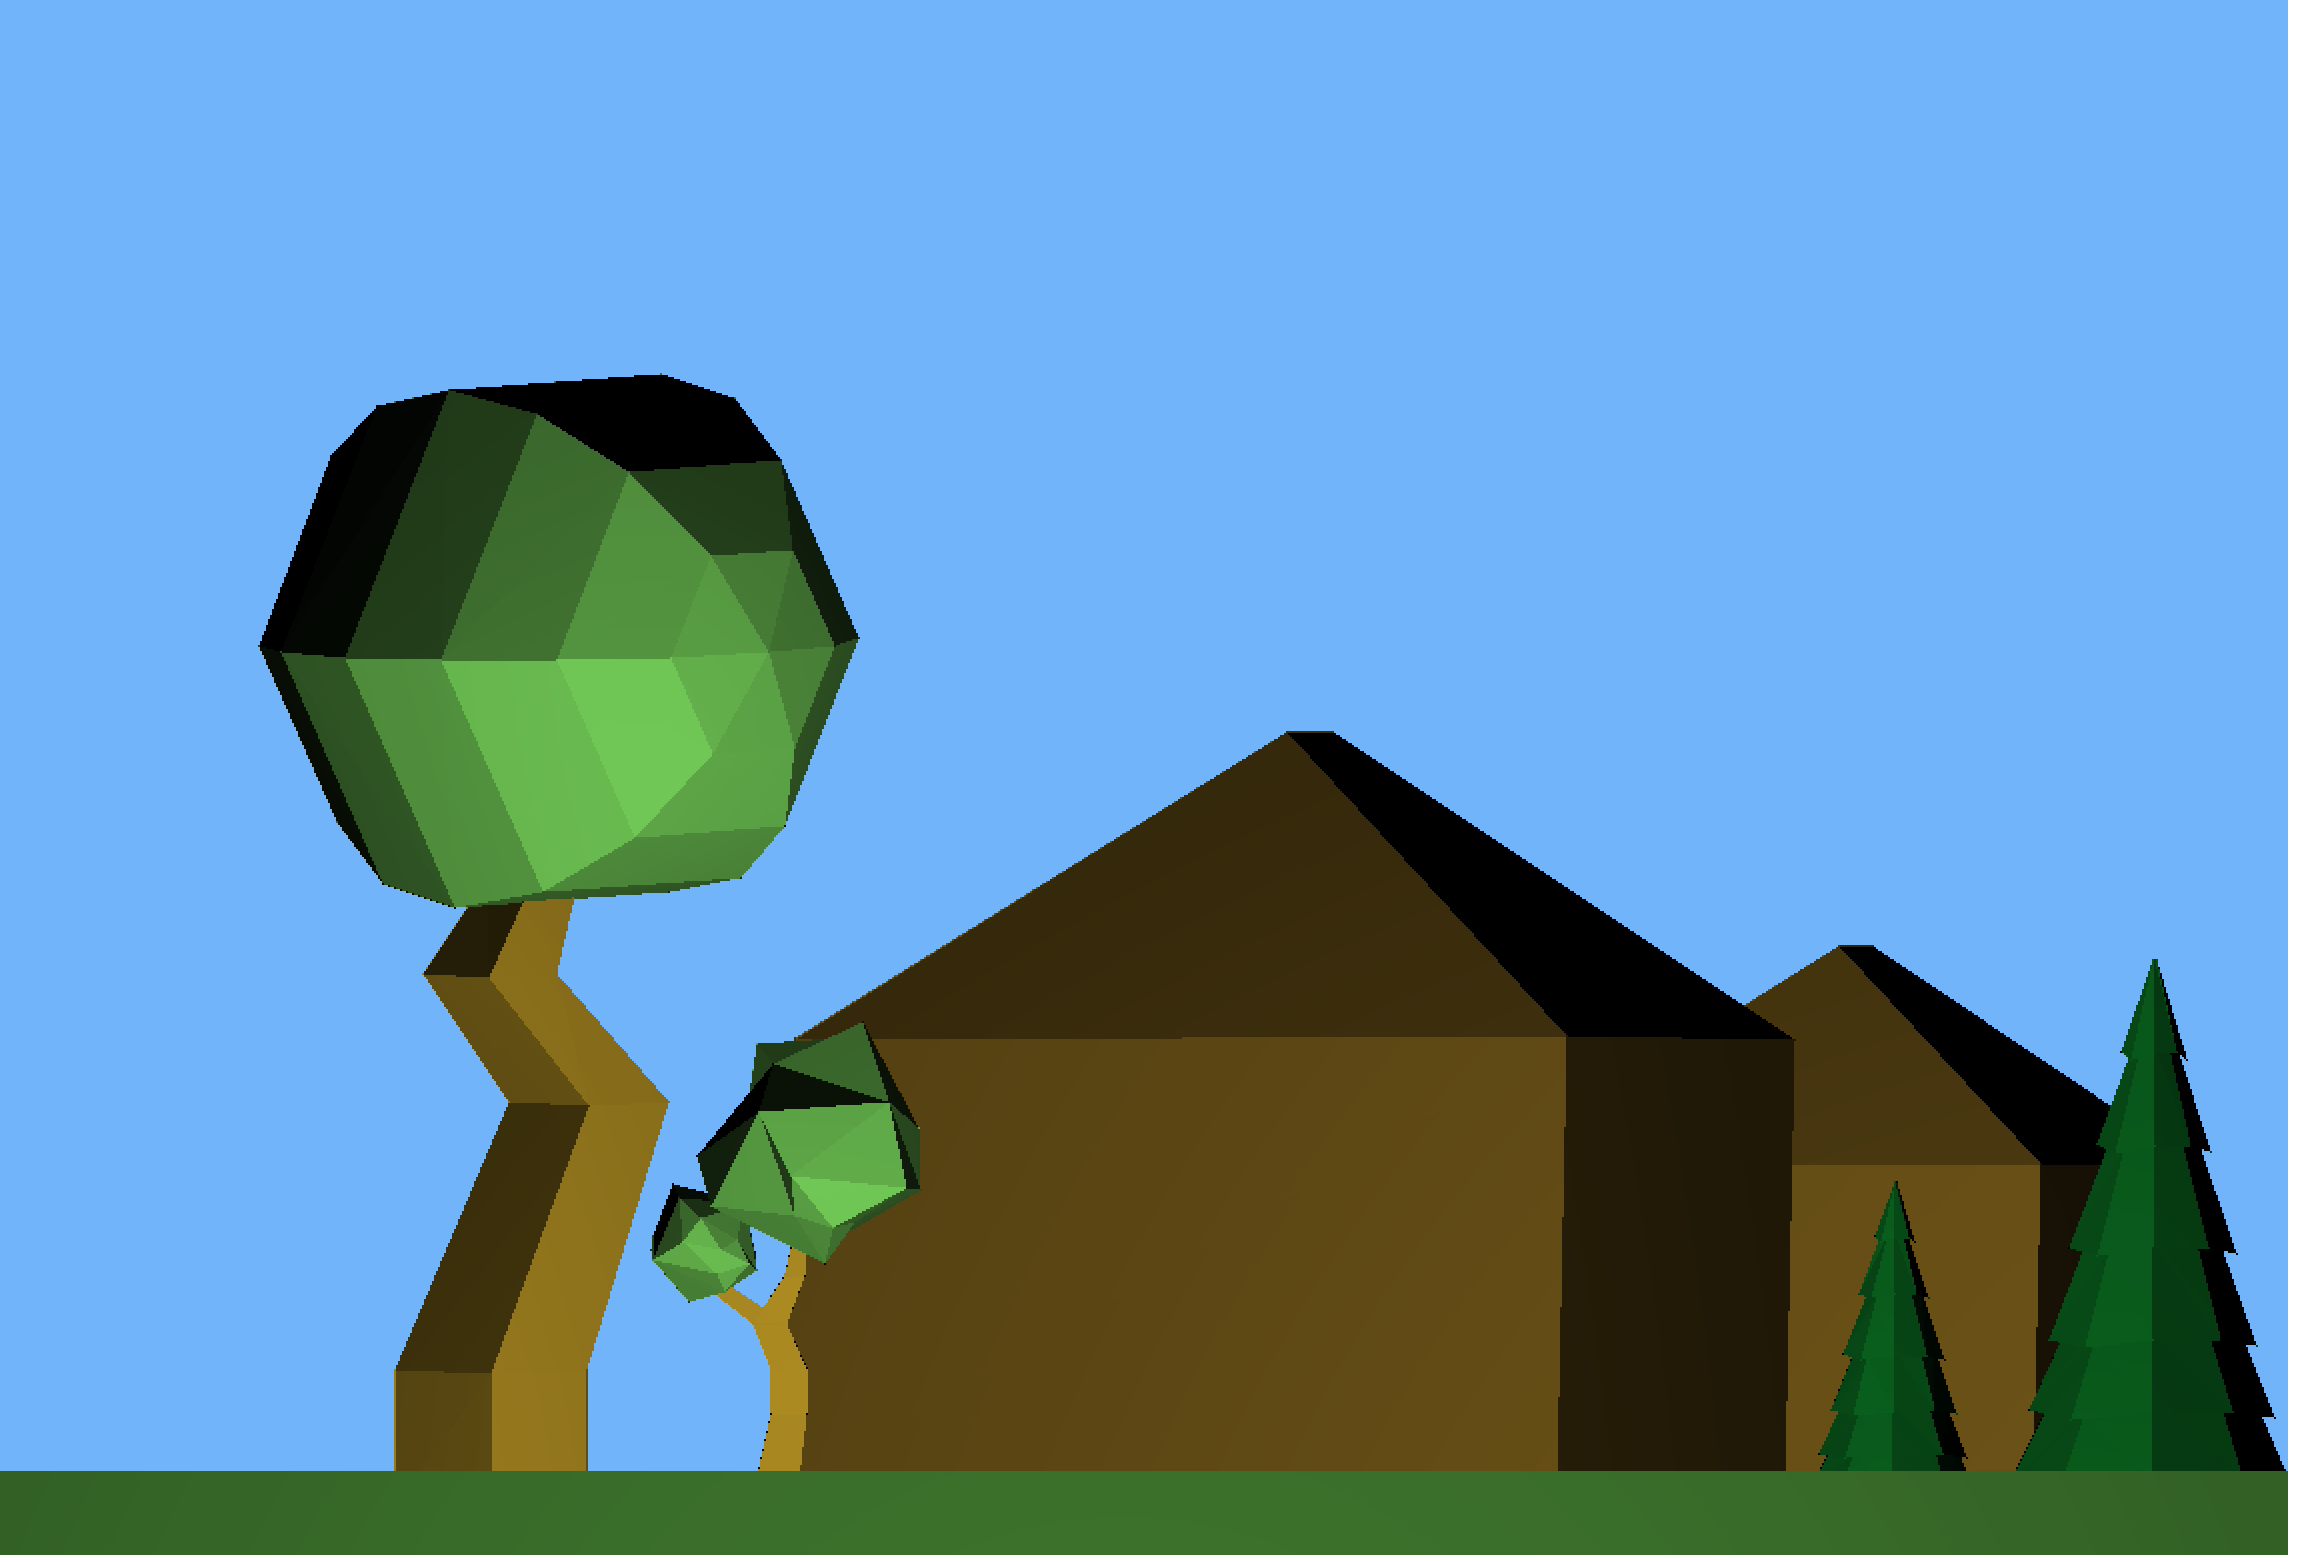
\includegraphics[scale=0.2]{include/1.png}
	\caption{Пример работы программы №1}
	\label{img:1}
\end{figure} 
\begin{figure}[H]
	\centering
	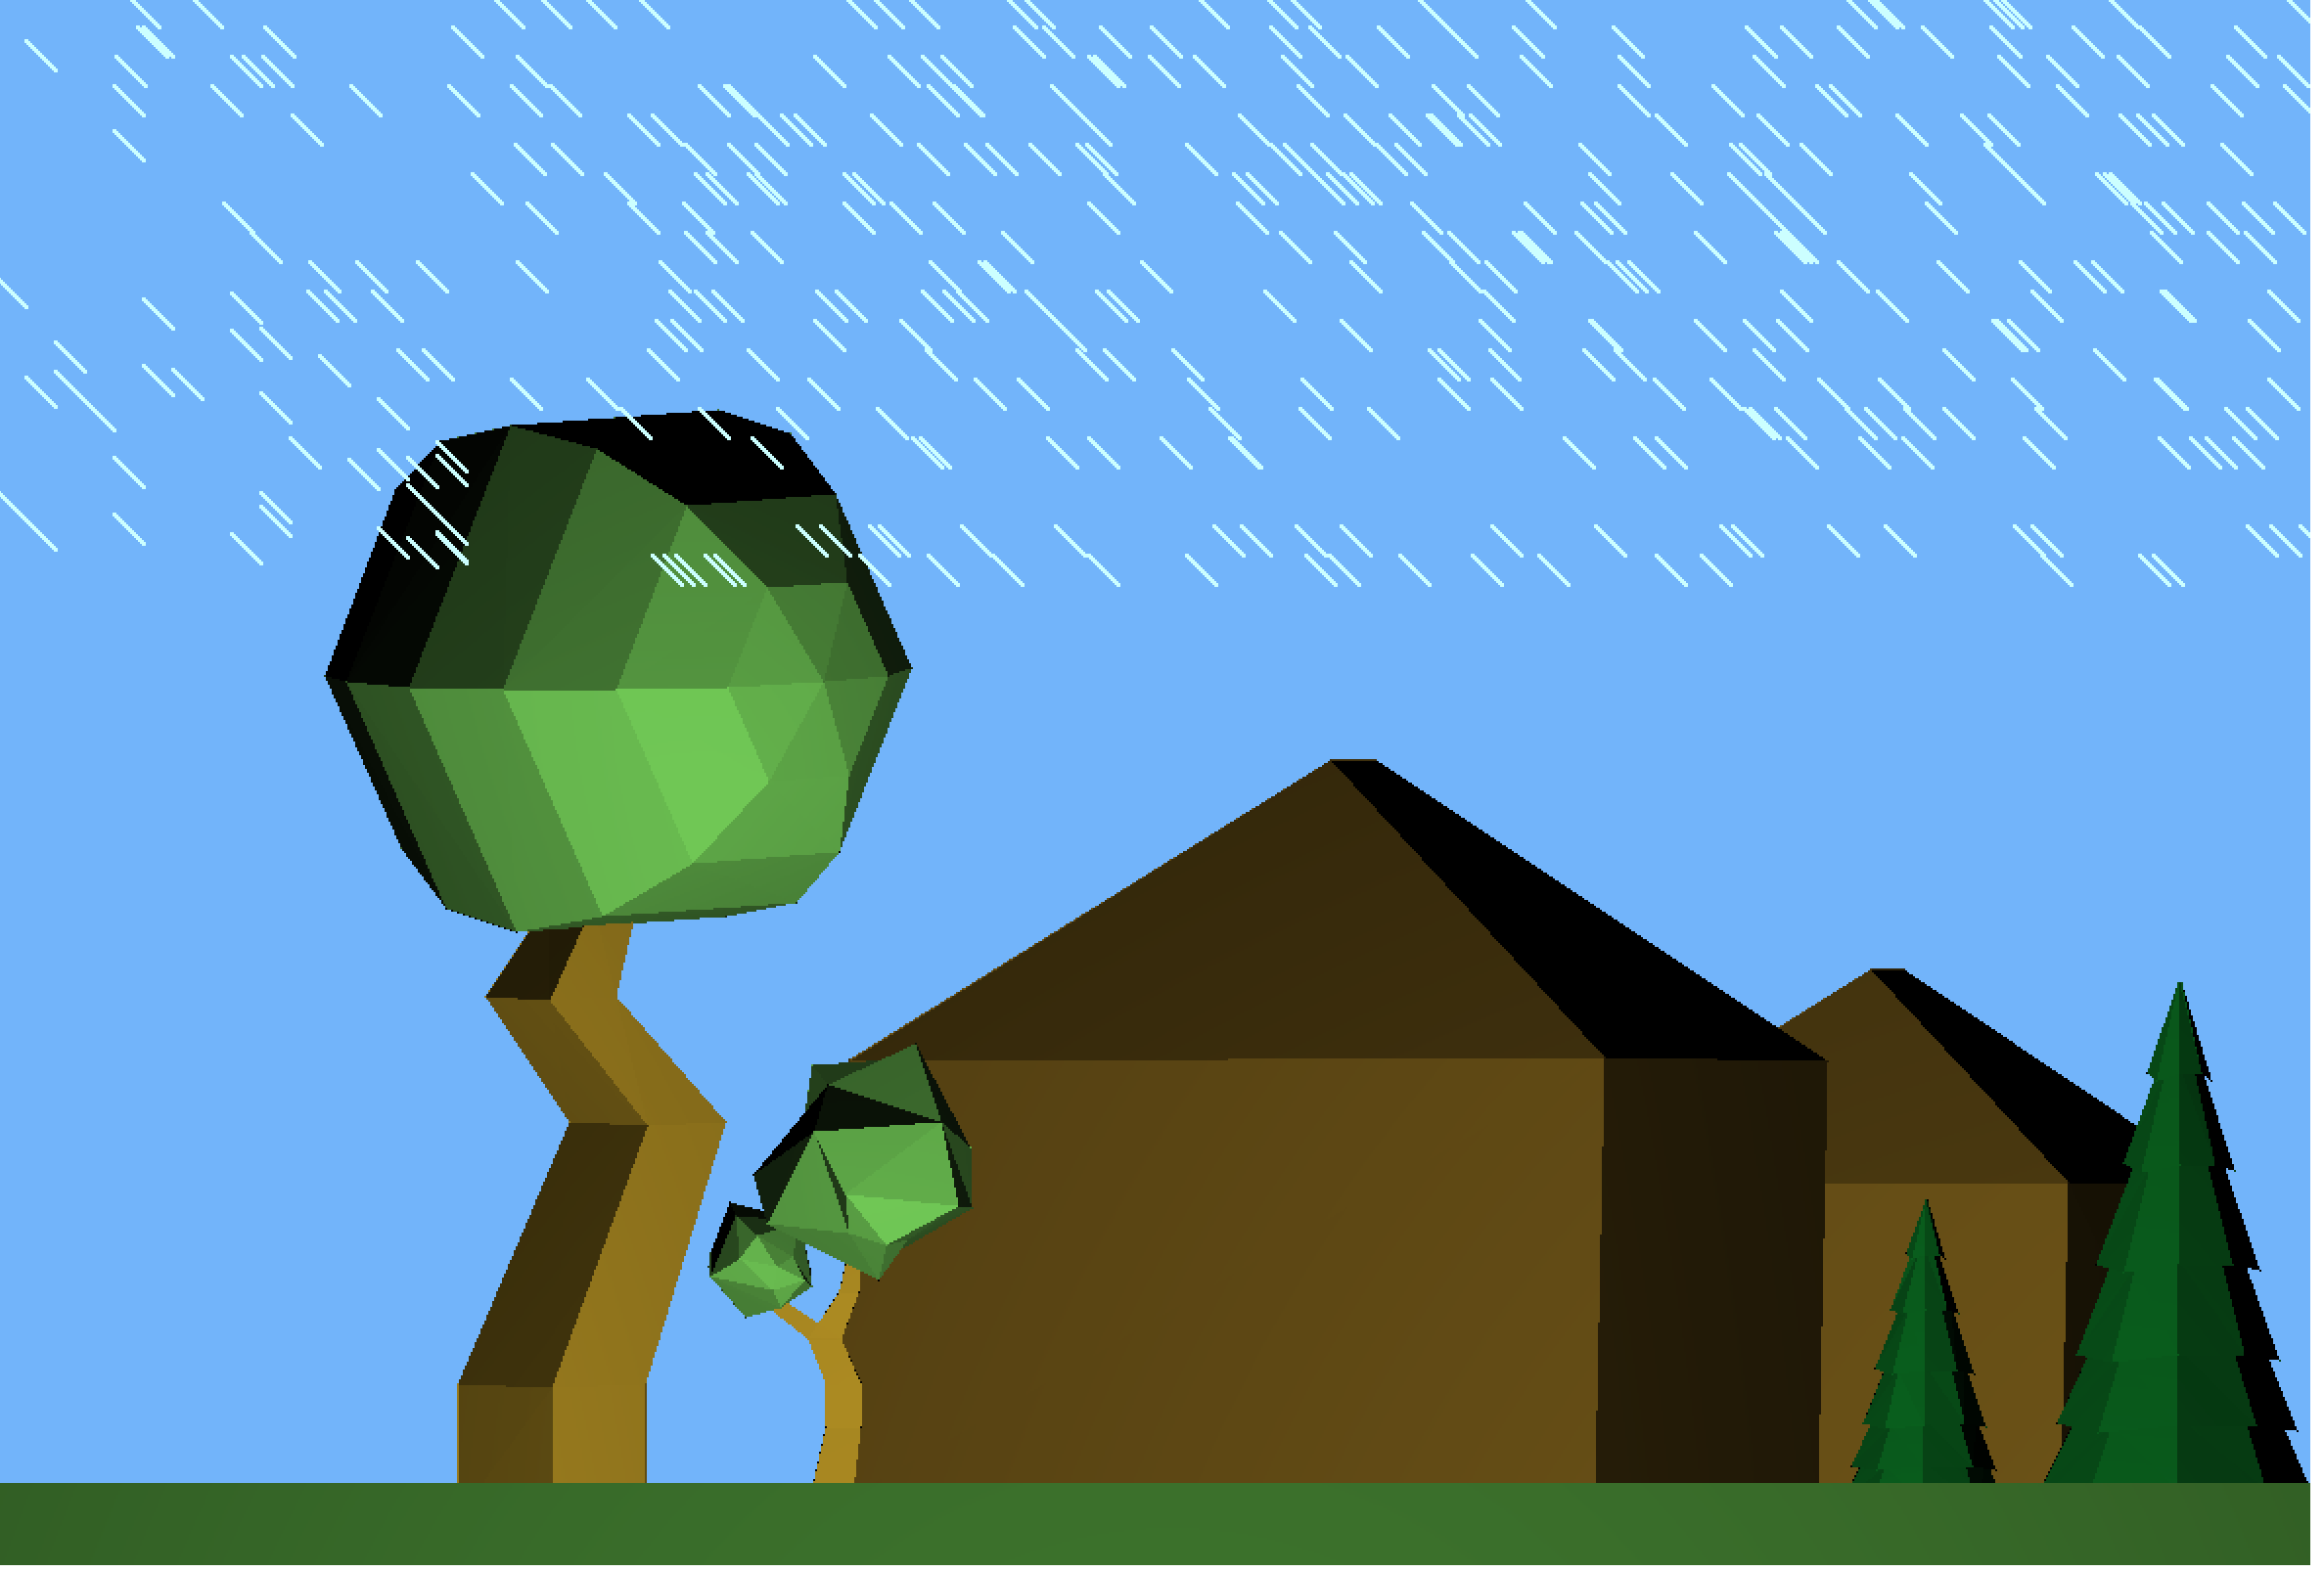
\includegraphics[scale=0.2]{include/2.png}
	\caption{Пример работы программы №2}
	\label{img:2}
\end{figure} 

\begin{figure}[H]
	\centering
	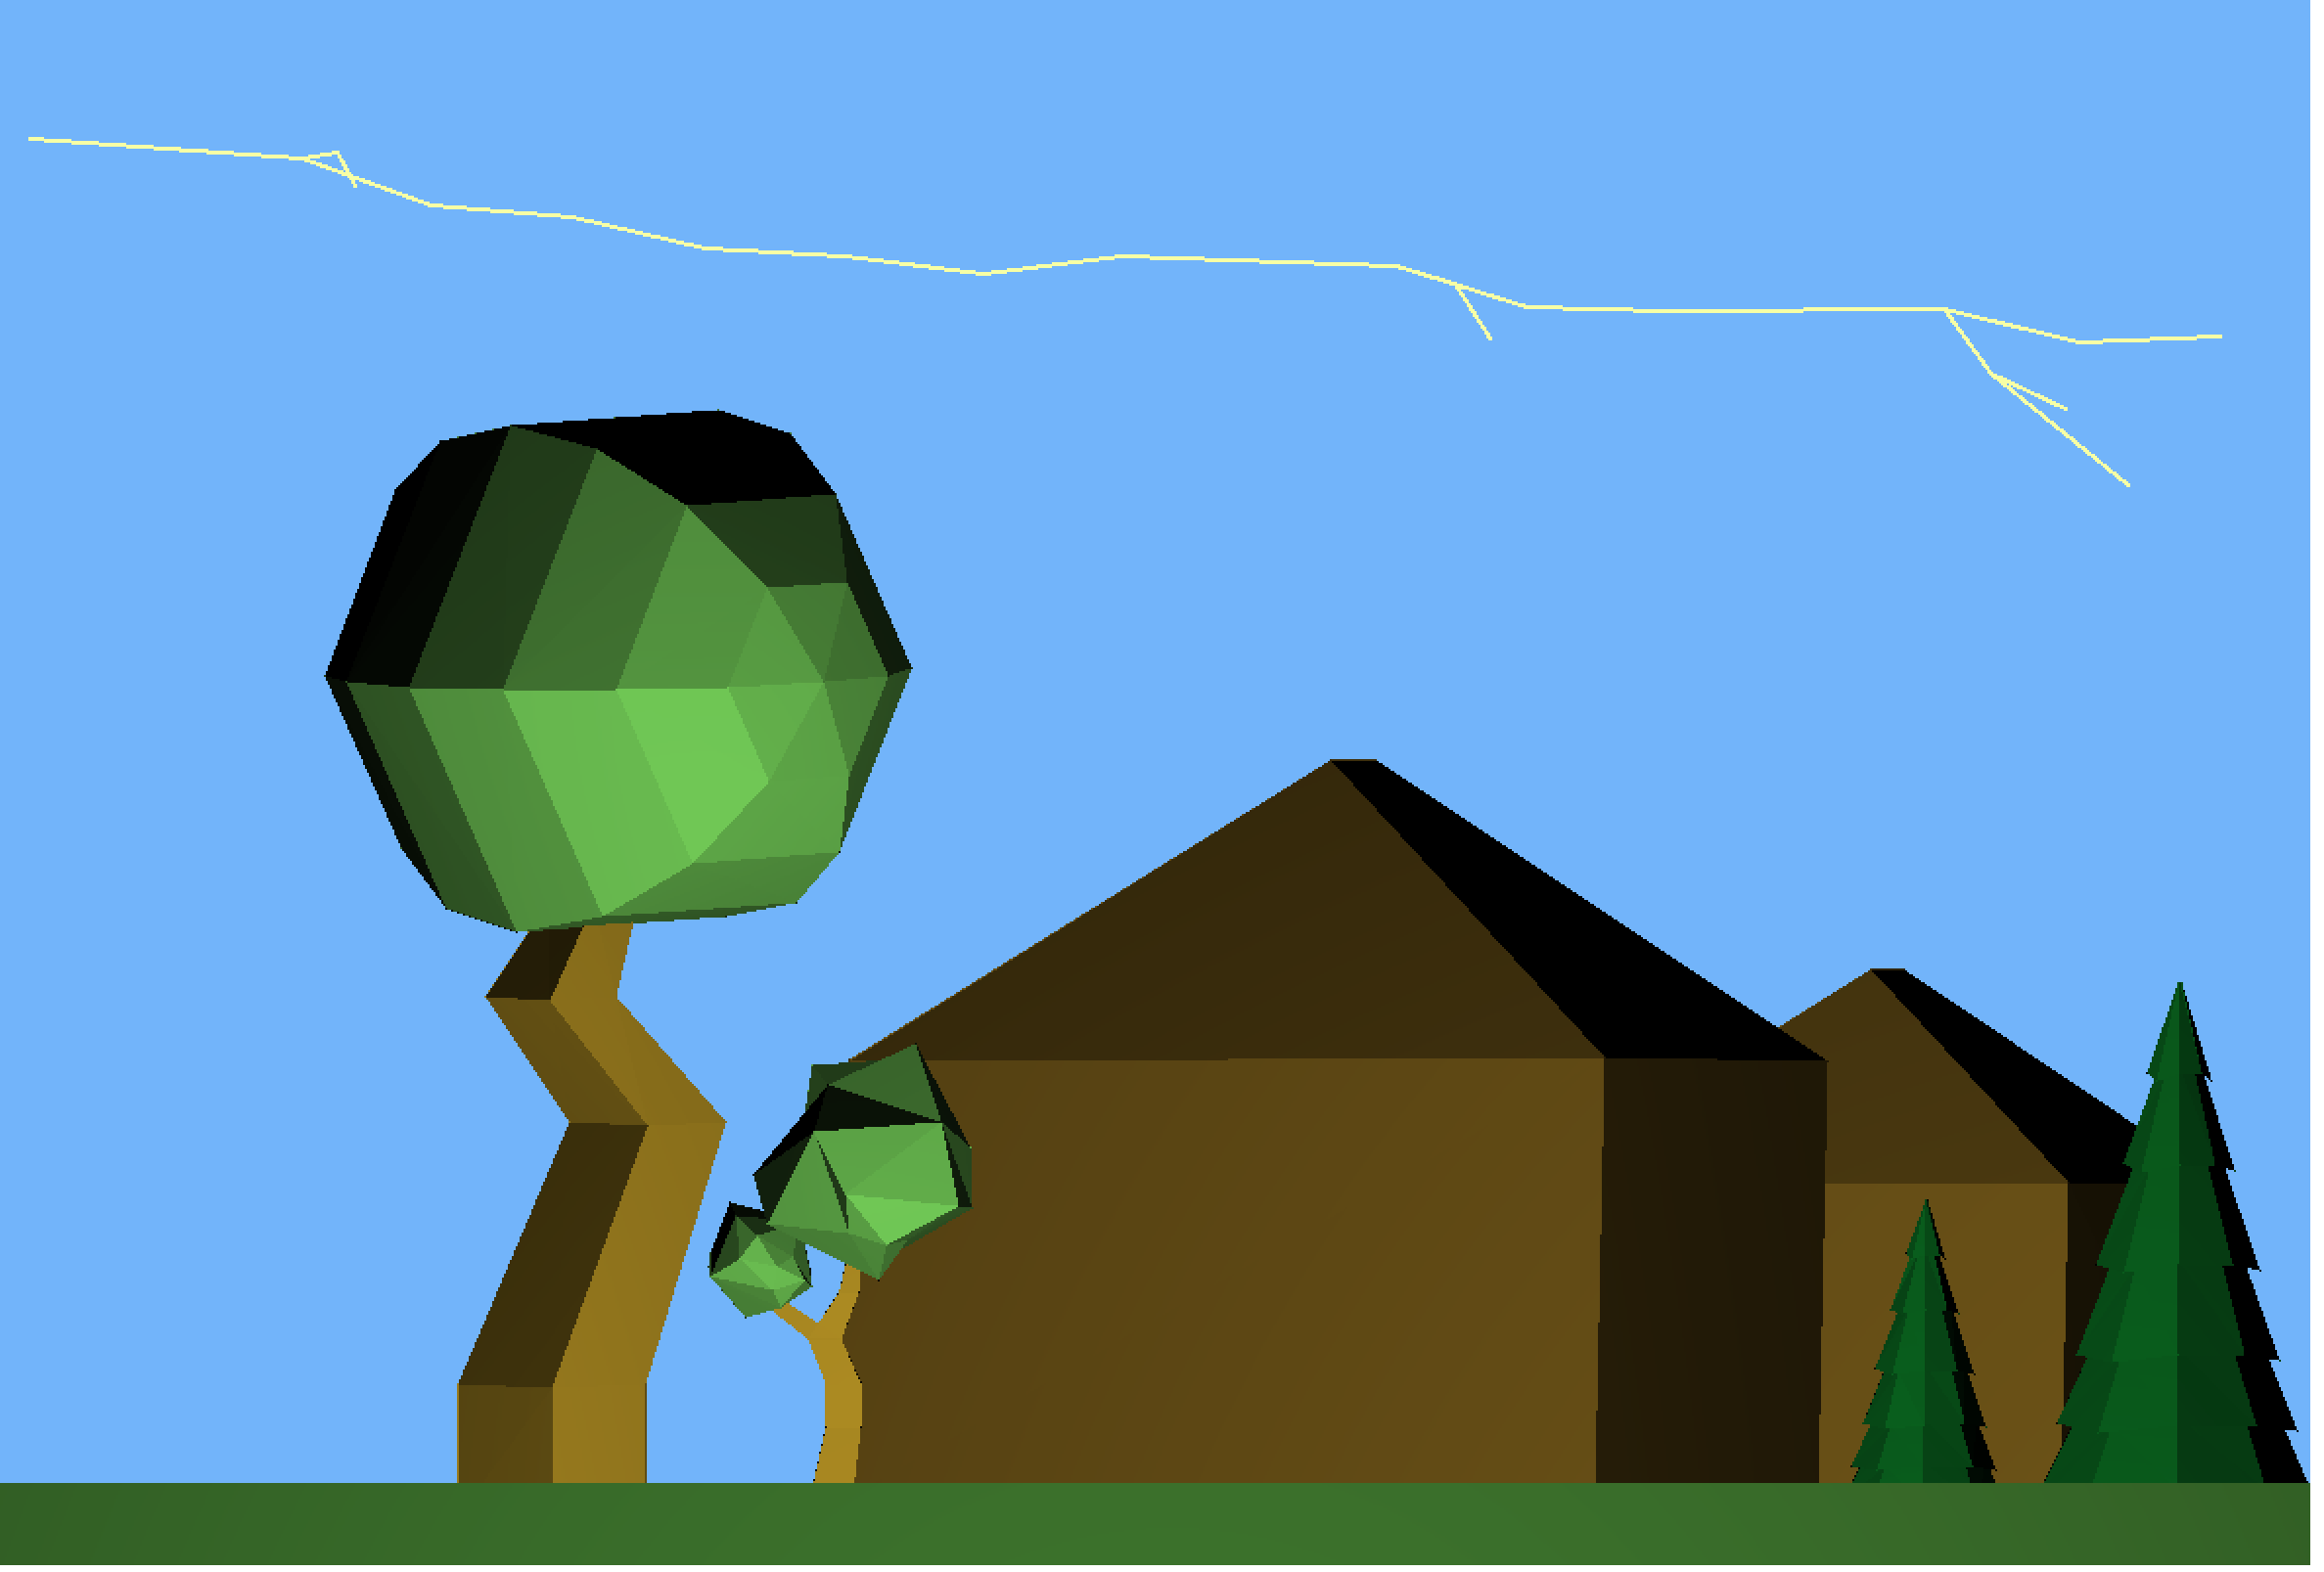
\includegraphics[scale=0.2]{include/3.png}
	\caption{Пример работы программы №3}
	\label{img:3}
\end{figure} 

\begin{figure}[H]
	\centering
	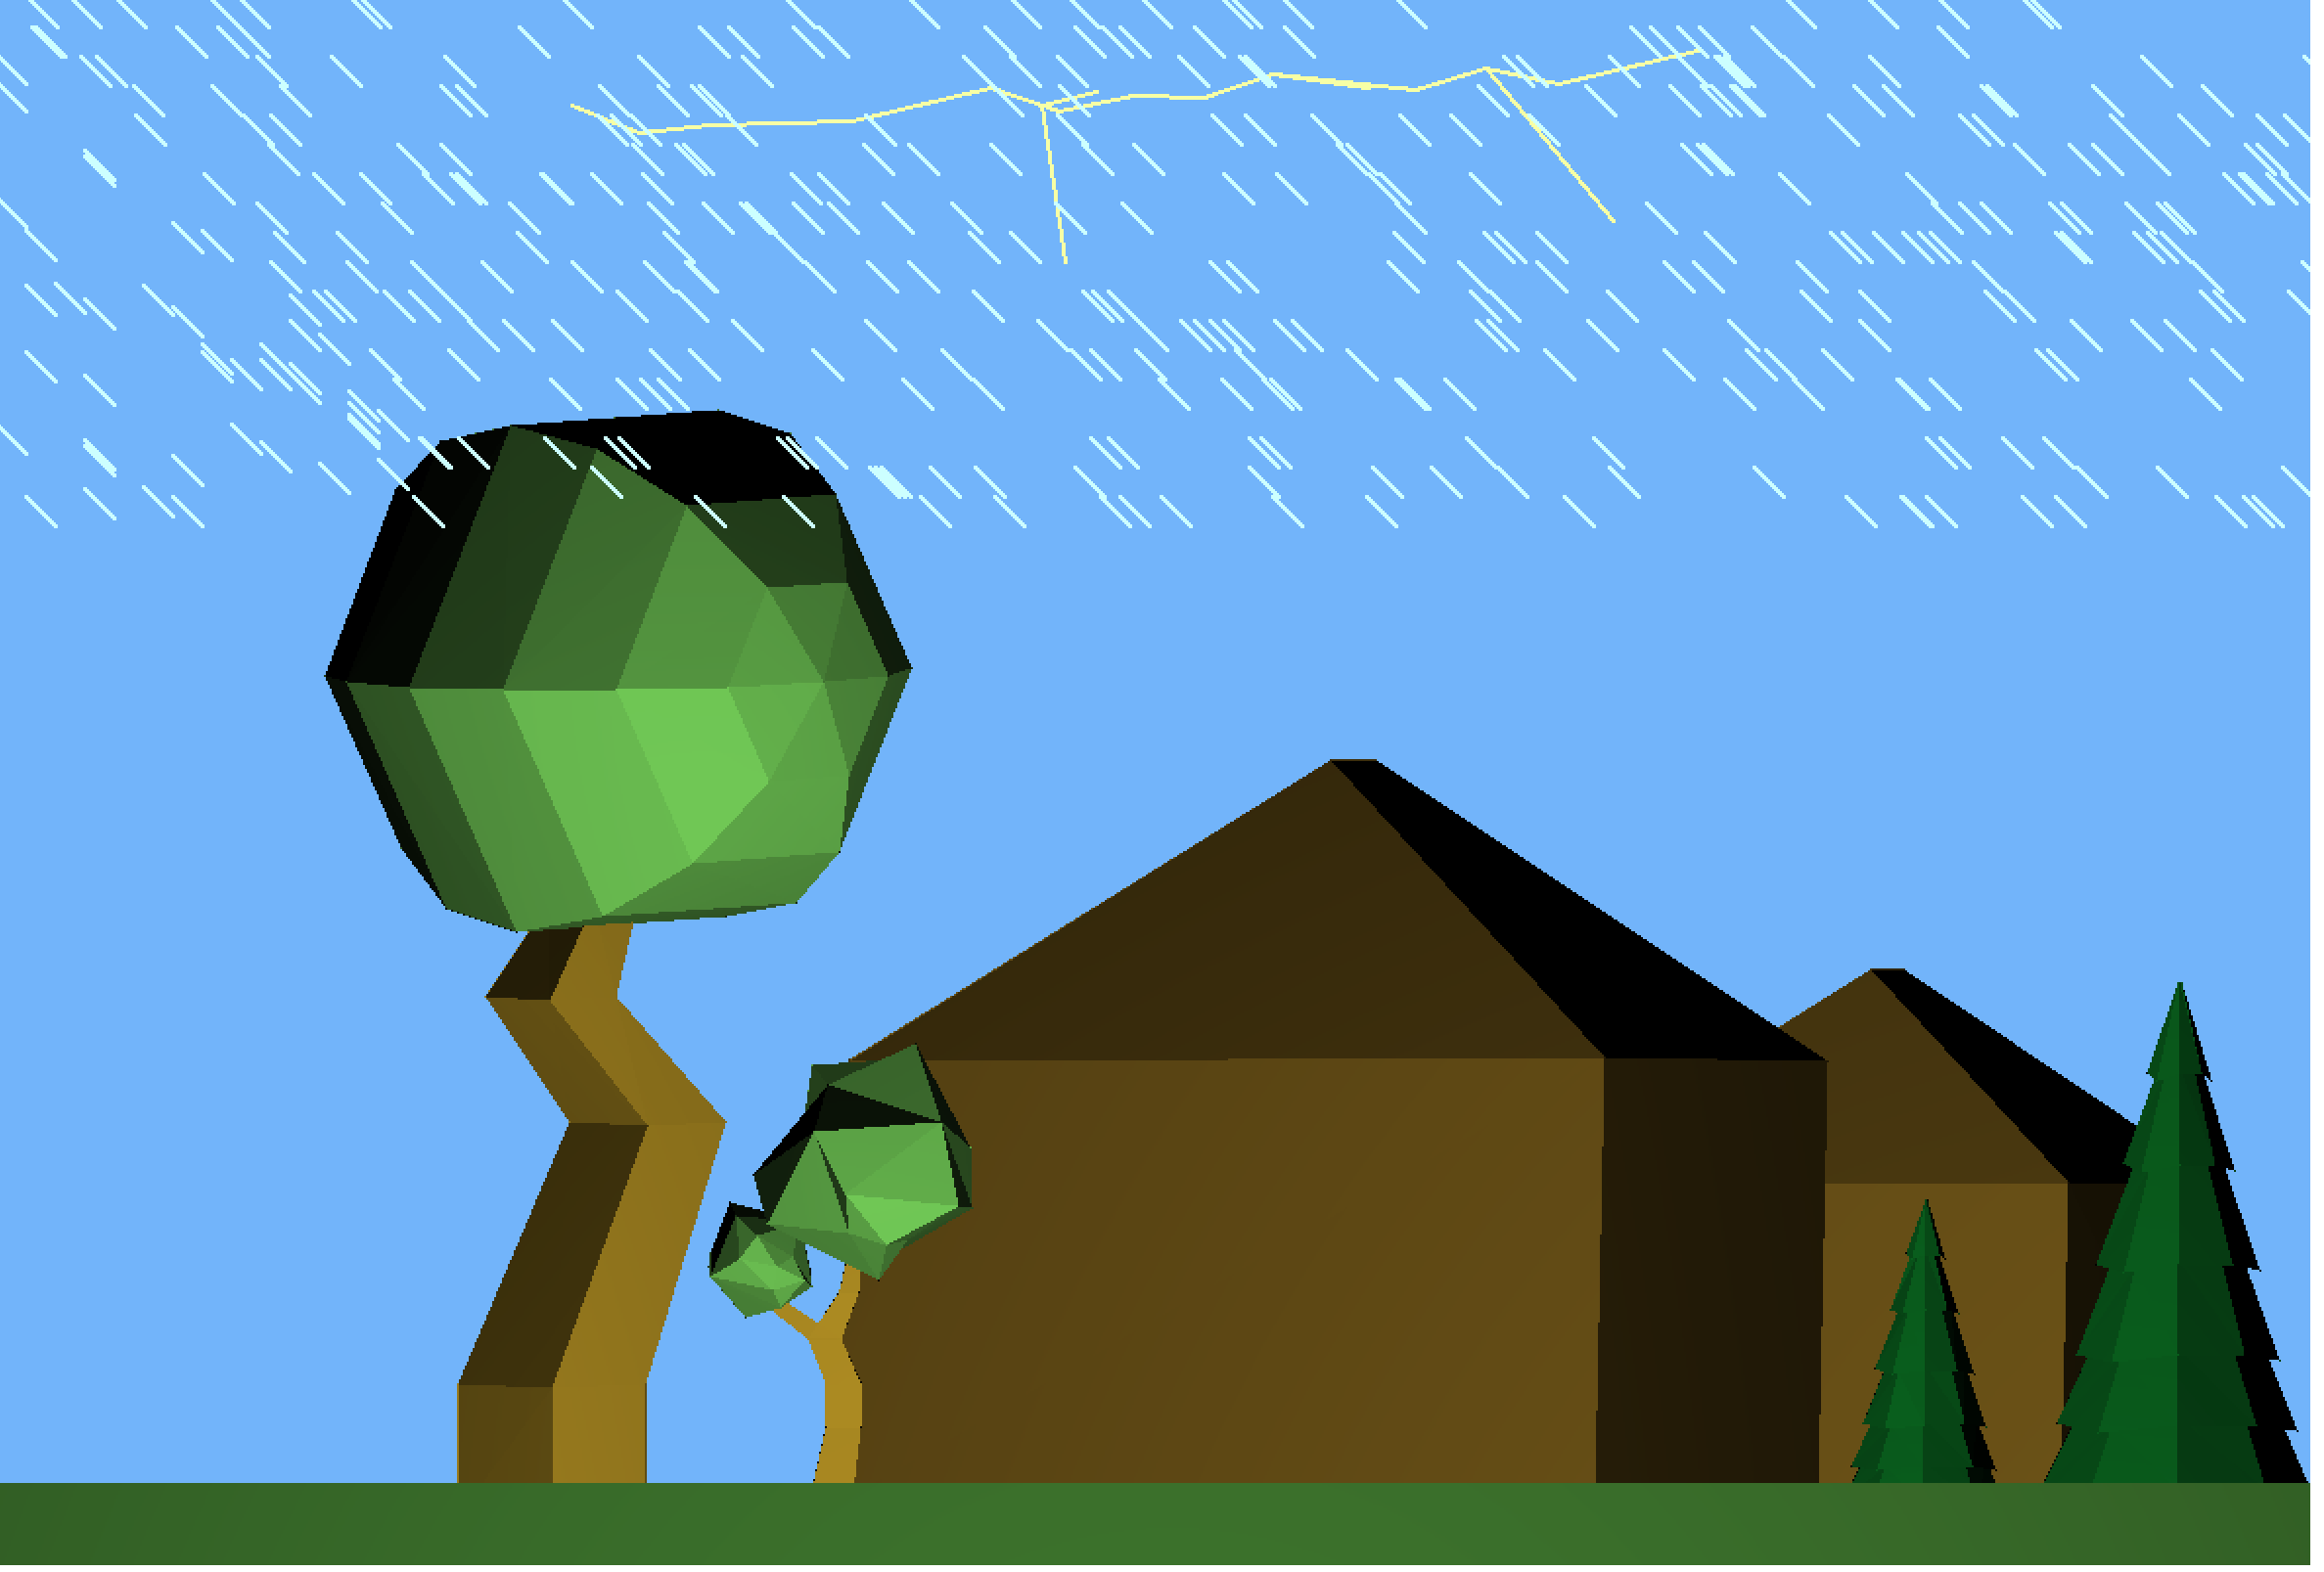
\includegraphics[scale=0.2]{include/4.png}
	\caption{Пример работы программы №4}
	\label{img:4}
\end{figure} 

\begin{figure}[H]
	\centering
	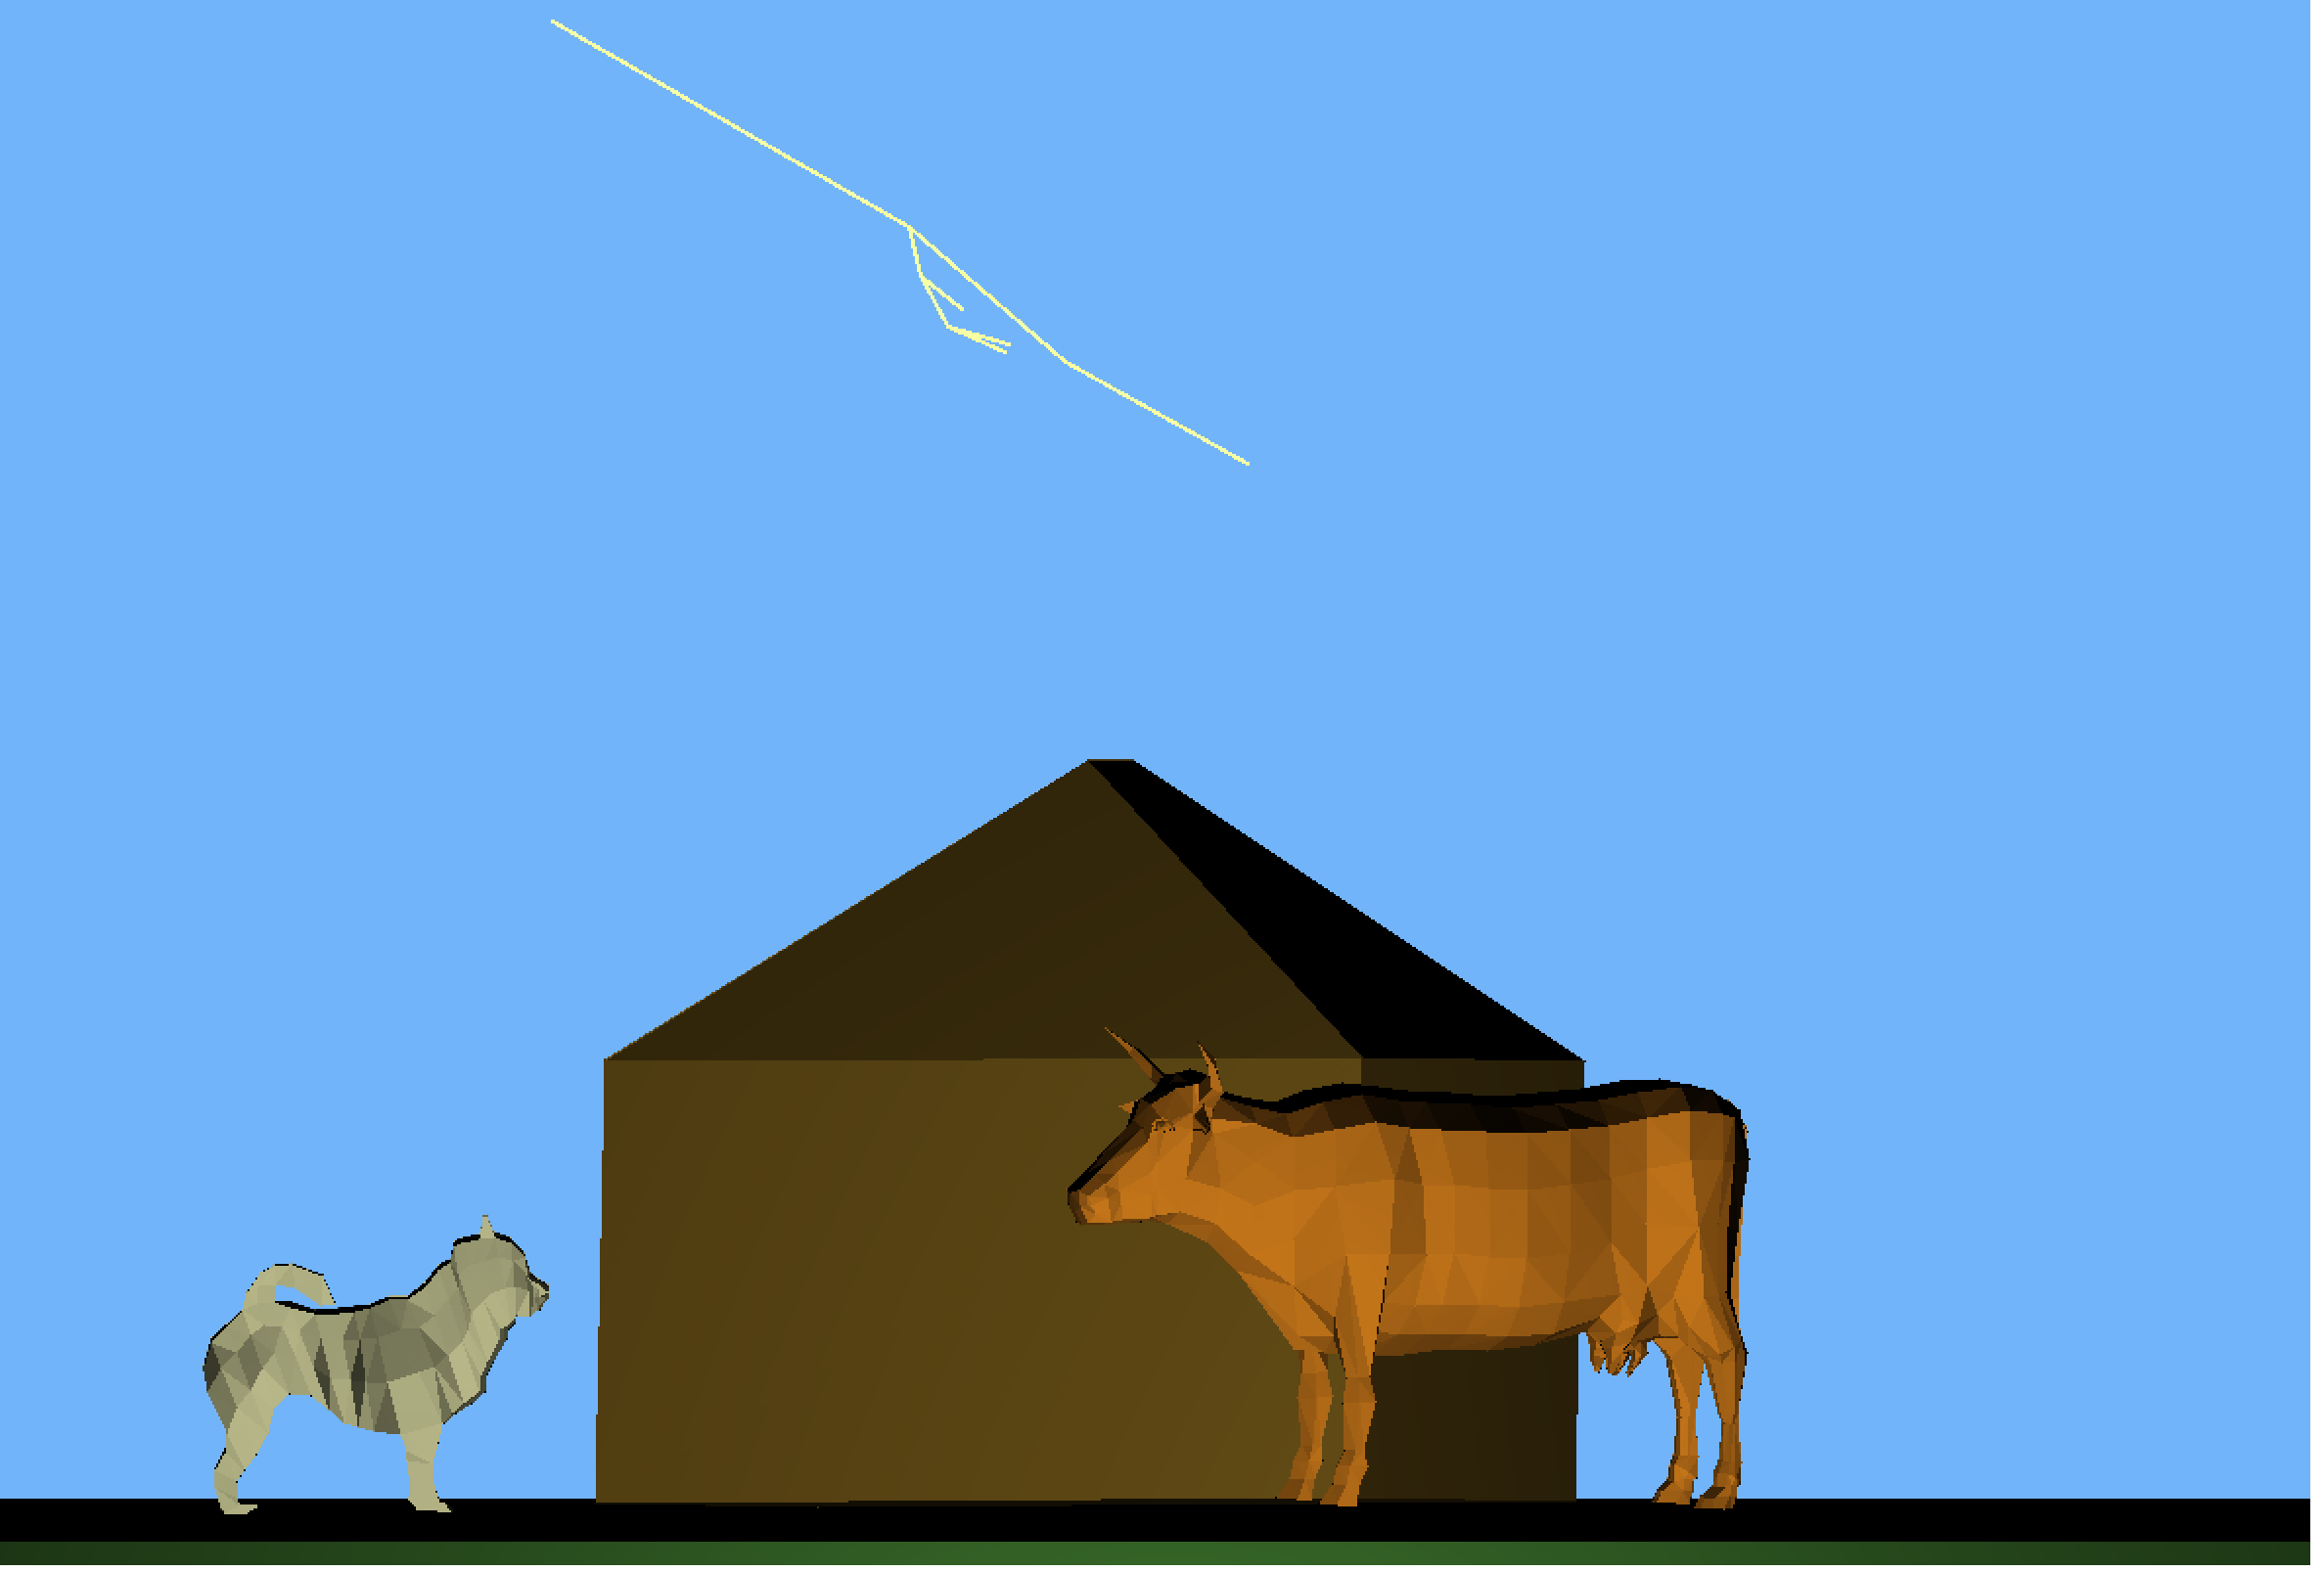
\includegraphics[scale=0.2]{include/5.png}
	\caption{Пример работы программы №5}
	\label{img:5}
\end{figure} 

\begin{figure}[H]
	\centering
	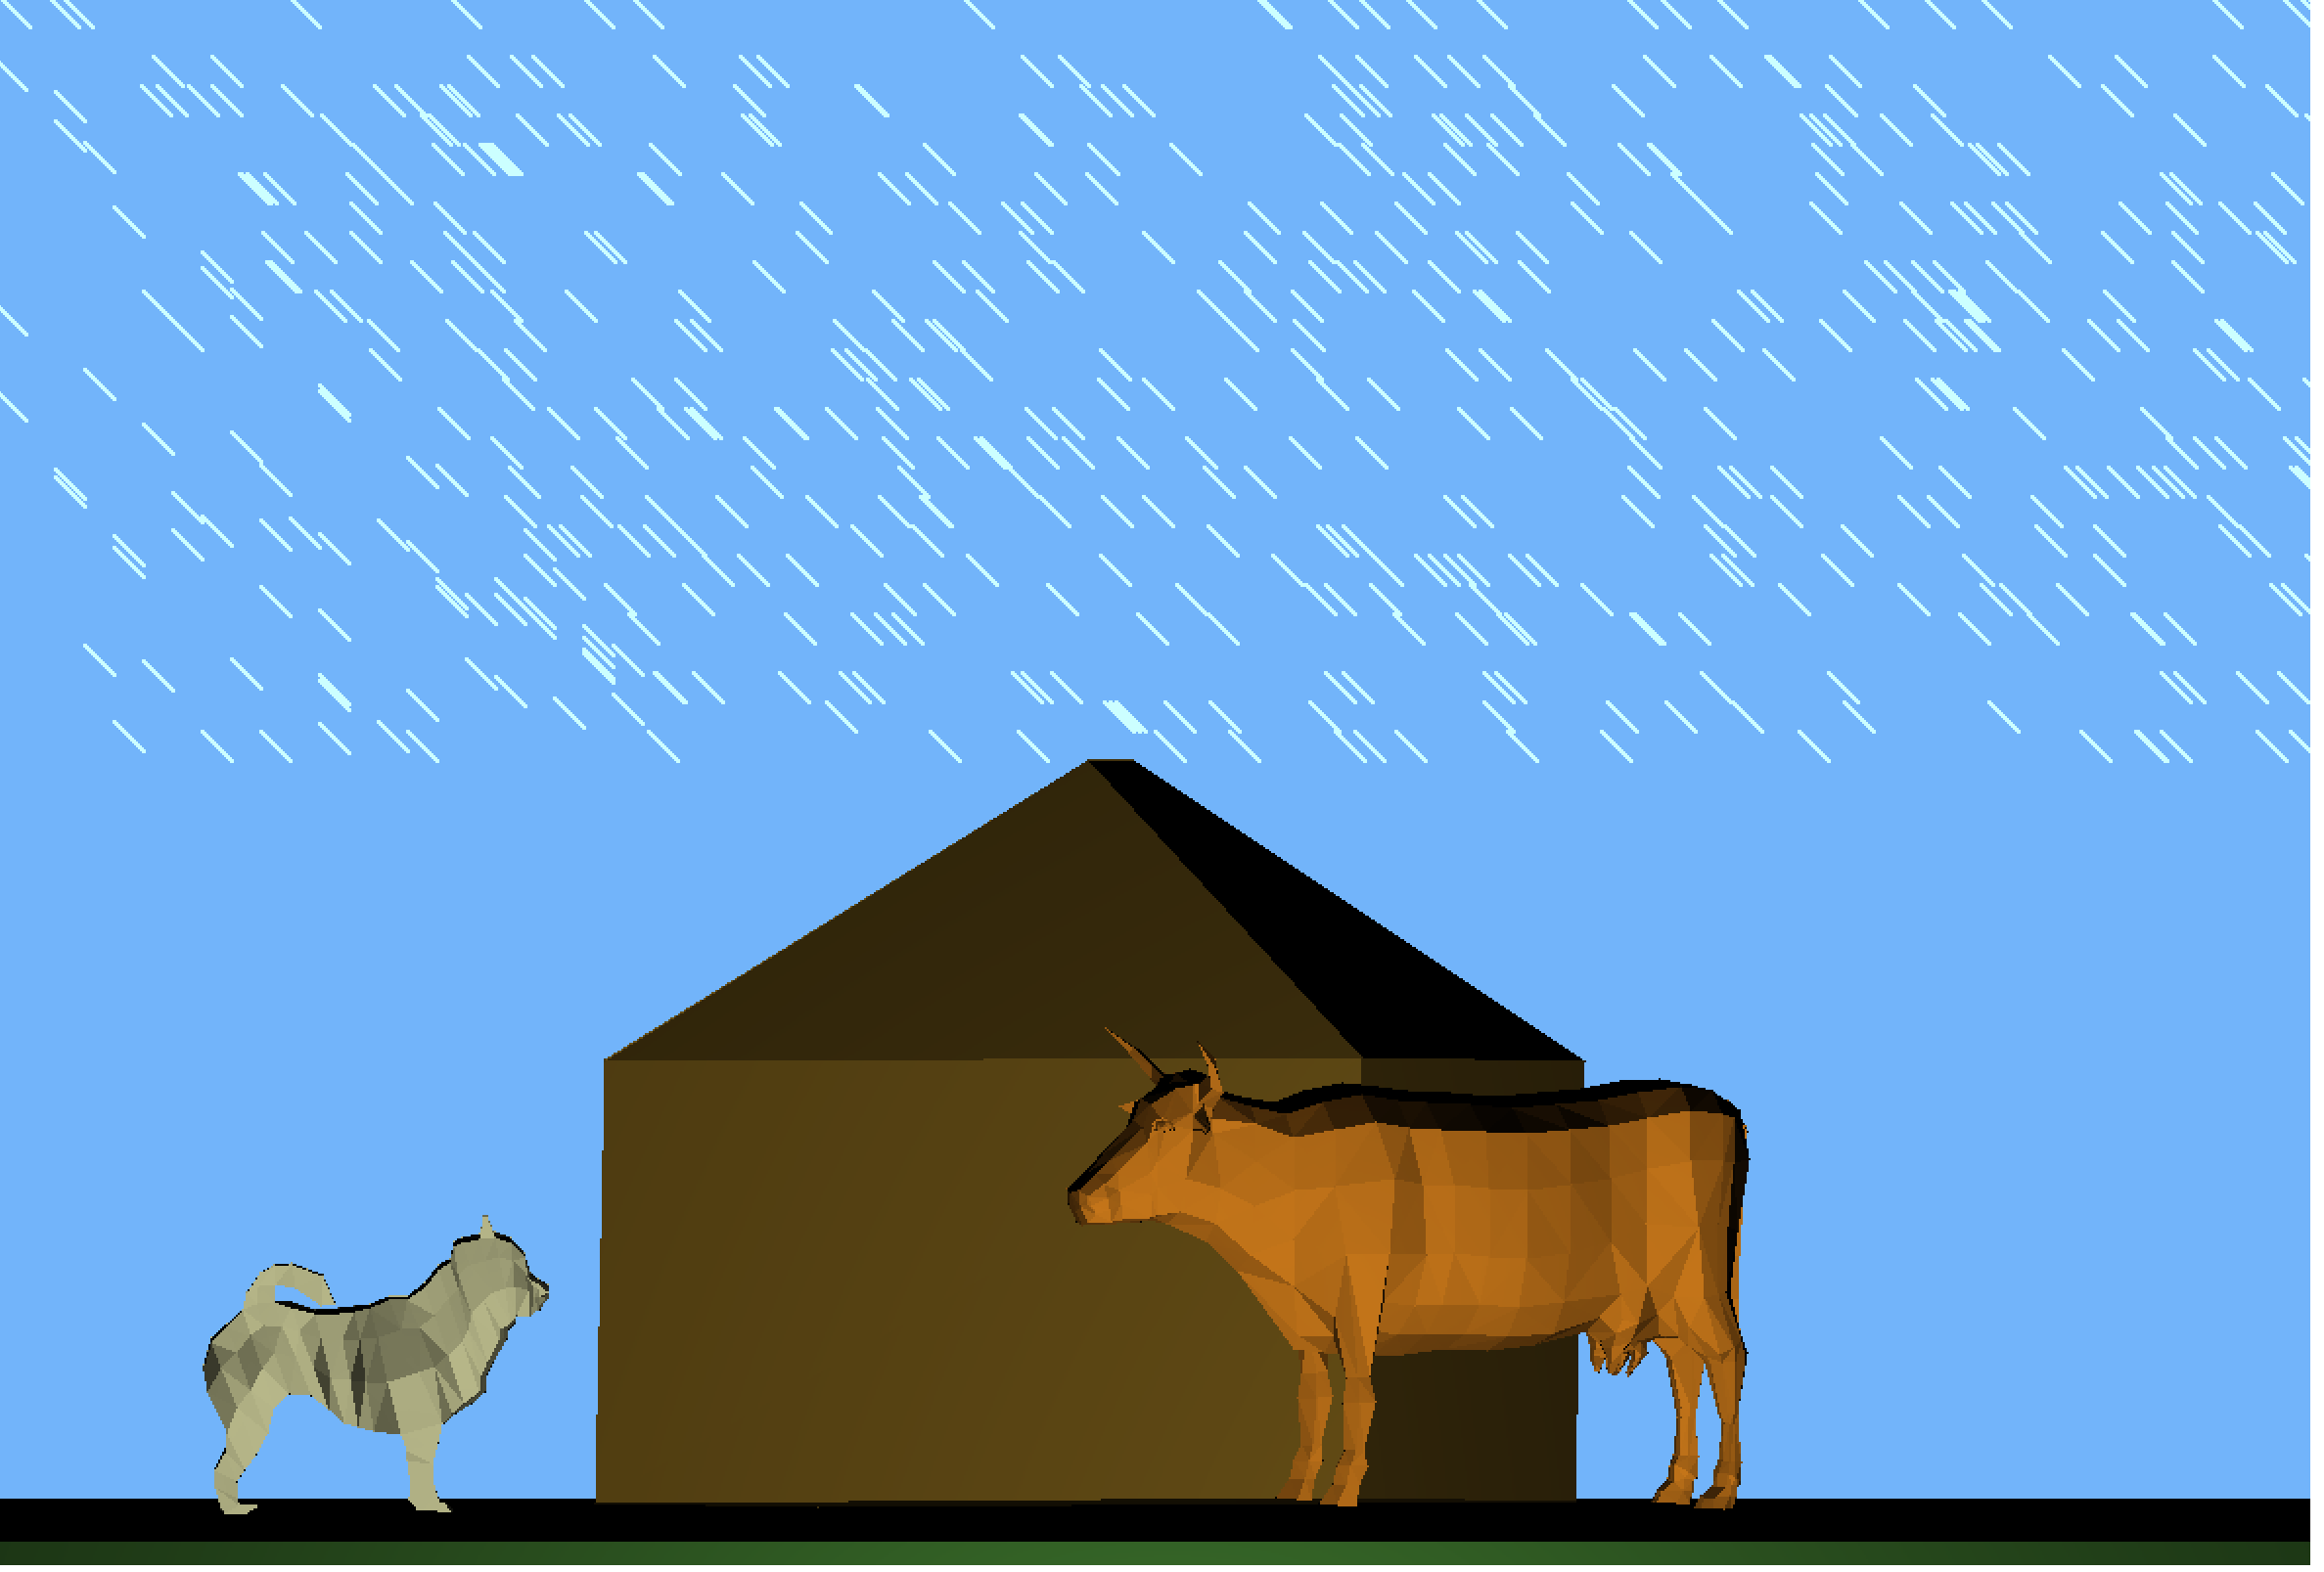
\includegraphics[scale=0.2]{include/6.png}
	\caption{Пример работы программы №6}
	\label{img:6}
\end{figure} 

\begin{figure}[H]
	\centering
	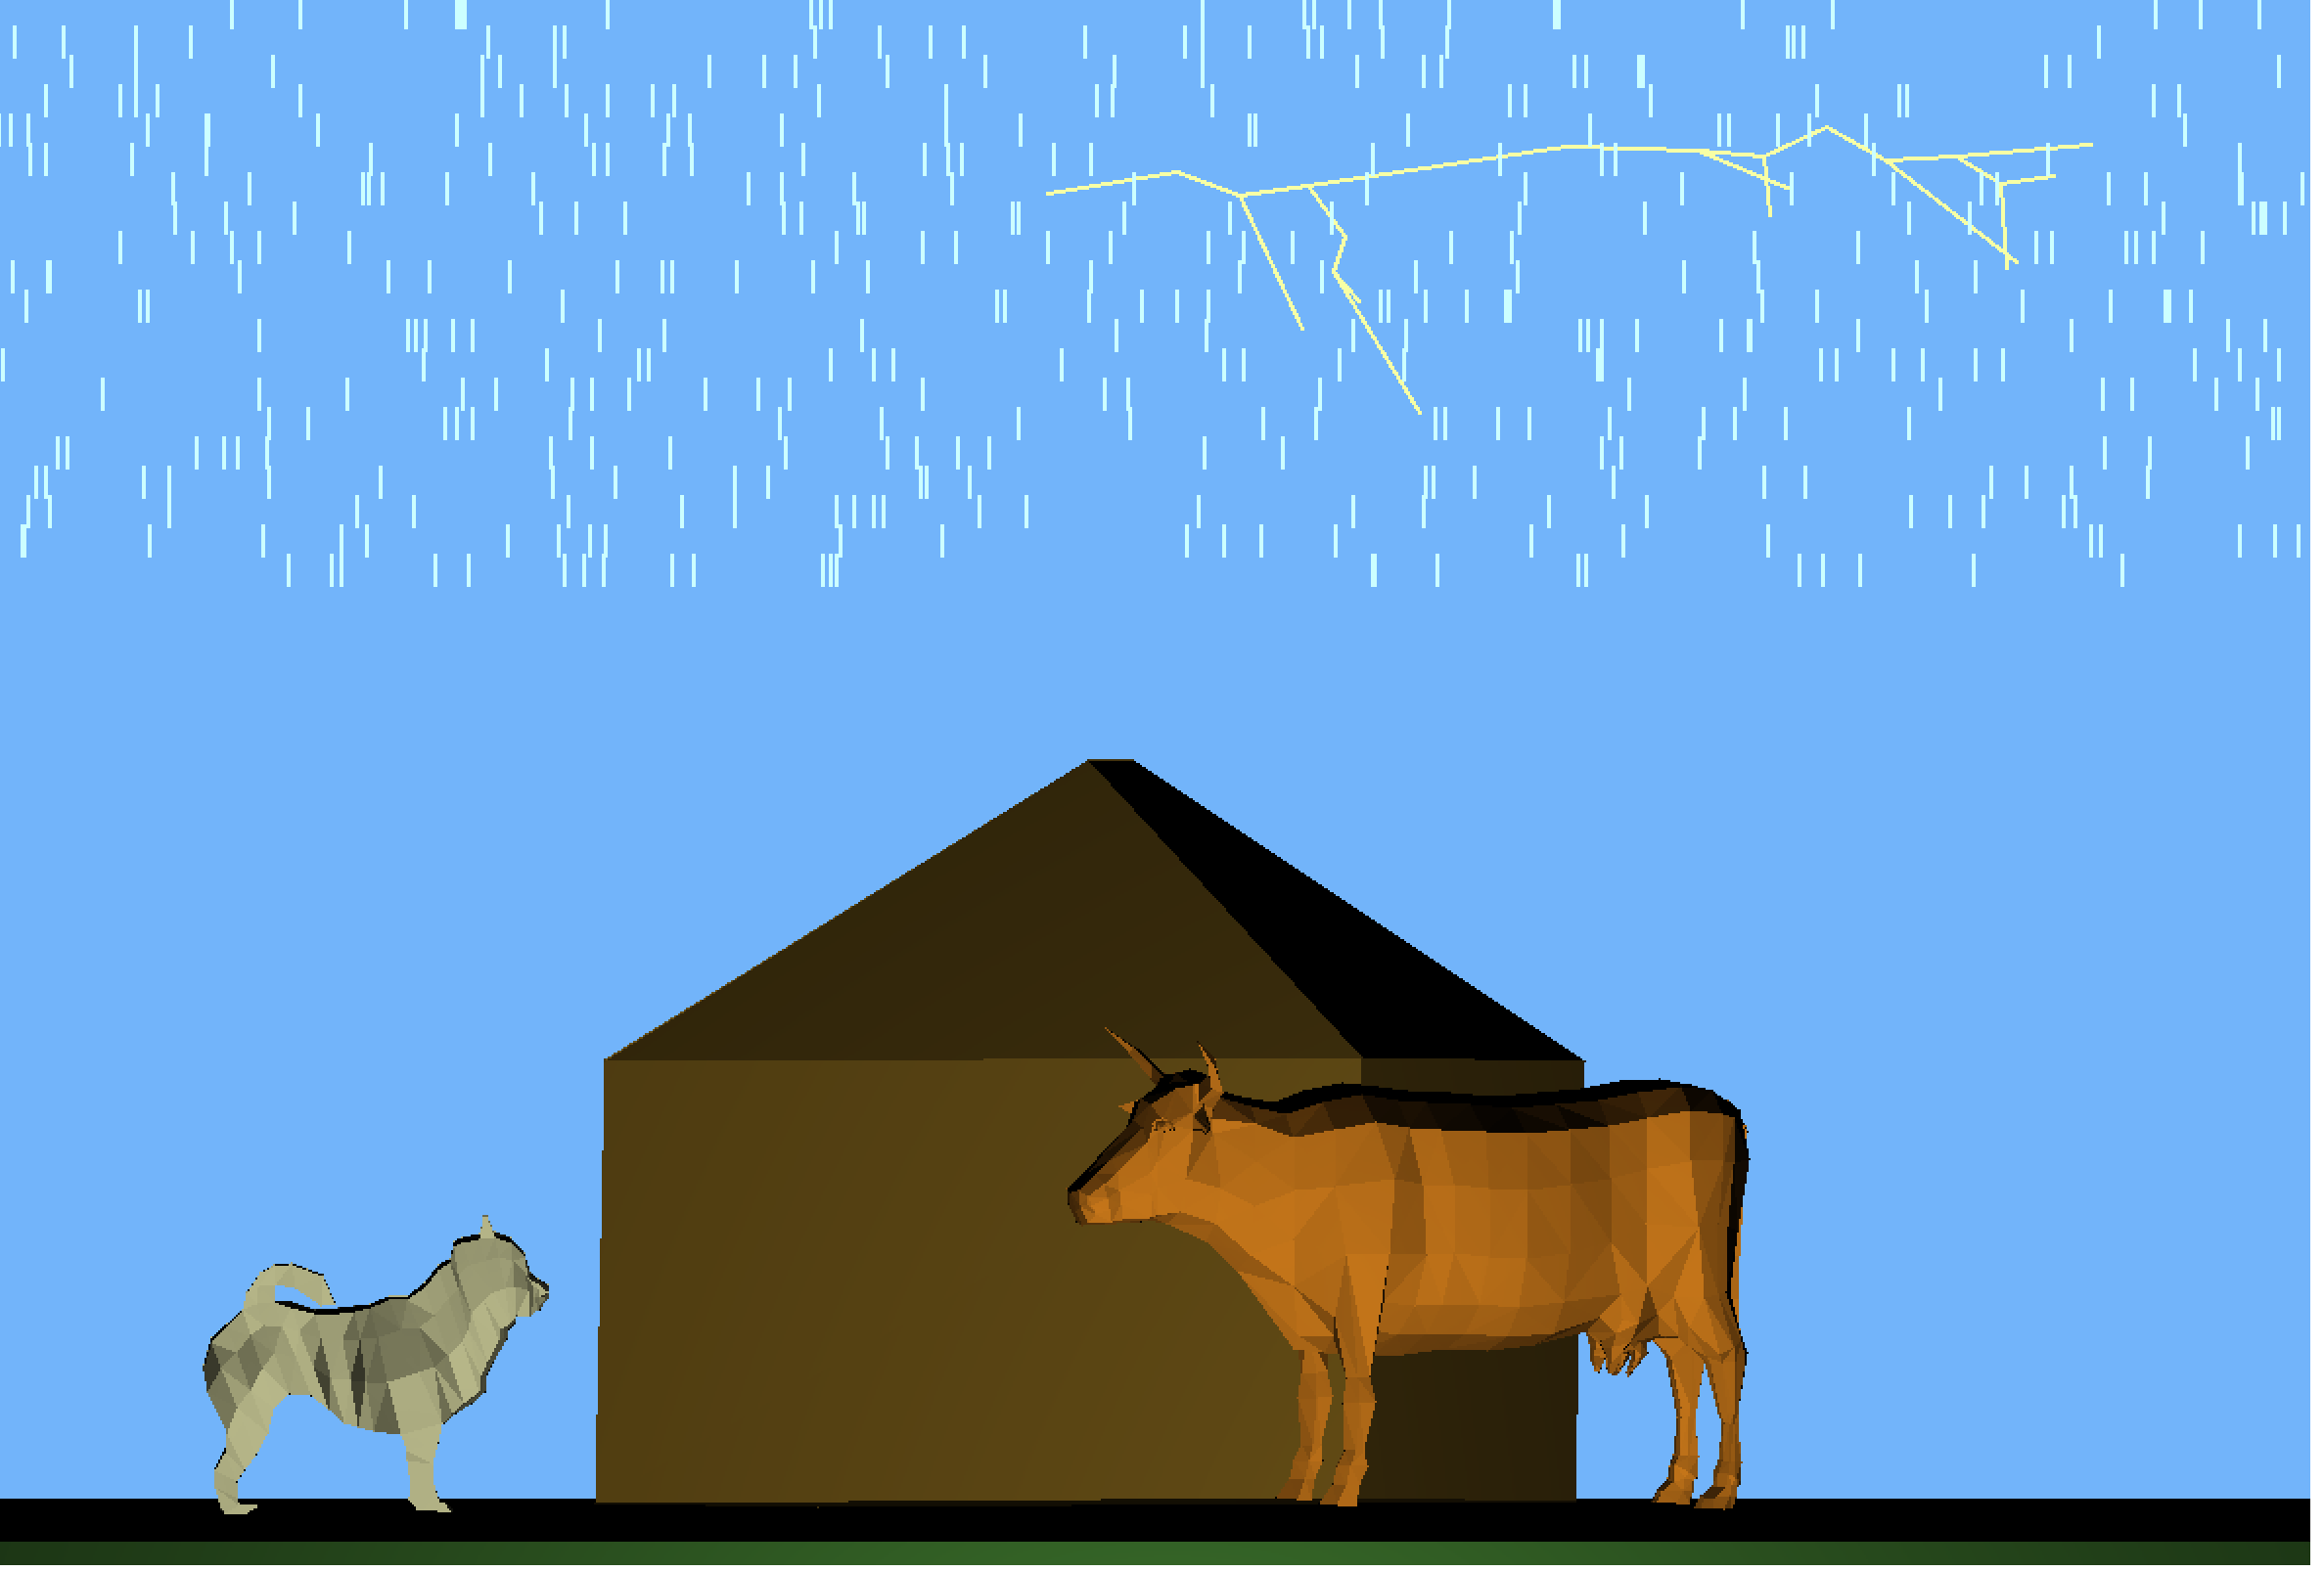
\includegraphics[scale=0.2]{include/7.png}
	\caption{Пример работы программы №7}
	\label{img:7}
\end{figure} 


\section{Вывод}

В данном разделе были рассмотрены средства реализации, описаны основные моменты
программной реализации, рассмотрен интерфейс программного продукта.